%% PLN credal degrees of freedom
%%
%% Render with:
%%   lualatex -shell-escape pln-credal-degrees-of-freedom.tex \
%%     && bibtex pln-credal-degrees-of-freedom \
%%     && lualatex -shell-escape pln-credal-degrees-of-freedom.tex \
%%     && lualatex -shell-escape pln-credal-degrees-of-freedom.tex

\documentclass[]{article}
\usepackage{url}
\usepackage[hyperindex,breaklinks,colorlinks=true,urlcolor=blue,linkcolor=black,citecolor=black]{hyperref}
\IfFileExists{breakurl.sty}{\usepackage{breakurl}}{}
\usepackage{xstring}
\usepackage{listings}
\lstset{basicstyle=\ttfamily\footnotesize,breaklines=true,frame=single,
        xleftmargin=1em,xrightmargin=0.5em}
\usepackage{float}
\restylefloat{table}
\usepackage{longtable}
\usepackage{booktabs}
\usepackage{graphicx}
\usepackage[font=small,labelfont=bf]{caption}
\usepackage[skip=0pt]{subcaption}
\usepackage{amsfonts}
\usepackage{amsmath}
\usepackage{amsthm}
\usepackage{tikz}
\usetikzlibrary{positioning,arrows.meta,calc,decorations.pathreplacing}
\usepackage{unicode-math}
\IfFileExists{newunicodechar.sty}{
  \usepackage{newunicodechar}
  \newunicodechar{∘}{\ensuremath{\circ}}
}{}
\IfFontExistsTF{Stix Two Math}{\setmathfont{Stix Two Math}}{\setmathfont{STIX Math}}

% Compatibility fallback for older TeX bundles.
\makeatletter
\providecommand{\headerps@out}{}
\makeatother

\newtheorem{theorem}{Theorem}
\newtheorem{lemma}[theorem]{Lemma}
\newtheorem{proposition}[theorem]{Proposition}
\newtheorem{corollary}[theorem]{Corollary}
\newtheorem{definition}[theorem]{Definition}
\newtheorem{remark}[theorem]{Remark}
\newtheorem{observation}[theorem]{Observation}

\newcommand{\nuPLN}{\texorpdfstring{$\nu$}{nu}\textup{PLN}}
\newcommand{\xiPLN}{\texorpdfstring{$\xi$}{xi}\textup{PLN}}
\newcommand{\code}[1]{\texttt{#1}}
\newcommand{\codepath}[1]{\path{#1}}
\newcommand{\lid}[1]{{\ttfamily\nolinkurl{#1}}}
% Repo path references auto-link to the public MeTTapedia GitHub.
% Lean sources live under lean/mettapedia/; papers/ is at the repo root.
\newcommand{\mpbase}{https://github.com/zariuq/MeTTapedia/blob/main/}
\newcommand{\lpath}[1]{%
  \IfBeginWith{#1}{Mettapedia/}%
    {\href{\mpbase lean/mettapedia/#1}{\texttt{\nolinkurl{#1}}}}%
    {\IfBeginWith{#1}{papers/}%
      {\href{\mpbase#1}{\texttt{\nolinkurl{#1}}}}%
      {\texttt{\nolinkurl{#1}}}}}
\newcommand{\ty}[1]{\ensuremath{\mathtt{#1}}}
\newcommand{\STV}[2]{\langle #1,\, #2 \rangle}
\newcommand{\strength}{\mathrm{strength}}
\newcommand{\confidence}{\mathrm{confidence}}
\newcommand{\Eq}{\;\Leftrightarrow\;}
% mini-diagram for each knob-zoo entry: uniform width + breathing room
\newcommand{\knobpic}[1]{\par\nopagebreak\vspace{3pt}%
  \centerline{\resizebox{0.5\linewidth}{!}{#1}}\vspace{6pt}\par}

\emergencystretch=3em

\title{Two numbers for a whole set of beliefs:\\
       what PLN's strength and confidence can and cannot see}
\author{Mettapedia Working Notes}
\date{\today}

\begin{document}
\maketitle

\begin{abstract}
A belief in PLN (Probabilistic Logic Networks) carries two numbers: a
\emph{strength} $s$ and a \emph{confidence} $c$. This paper explains, from
scratch, what those two numbers really stand for and exactly when they tell the
whole story. The short version: behind the pair $\STV{s}{c}$ sits a whole
\emph{set} of probability assignments you have not yet ruled out; strength is
the centre of that set on the question you asked, and confidence measures how
narrow the set is. Two numbers are a faithful summary of the set when the set
pins your question down to a single value, and a lossy summary when the set
leaves a genuine \emph{interval} of admissible answers.

We make this precise with a single recurring picture --- \emph{pinned} versus a
\emph{range} --- and follow it up three rising levels: one belief; a belief
built from many local pieces; and three infinite limits (order-free data
streams; weakly coupled systems, which collapse to one precise answer; and
strongly coupled systems, where distant conditions keep a real interval open).
Along the way we catalogue nineteen design choices --- ``degrees of freedom''
--- that two numbers either expose or hide, each with a numeric example
you can run. Every claim has a machine-checked counterpart; the formal
statements are collected, de-jargoned, in an appendix, and a runnable example
pack reproduces every number in the paper.
\end{abstract}

\tableofcontents

\section{One flip versus a hundred}\label{sec:hook}

You flip a bent coin once and it lands heads. \emph{One out of one --- so far it
always comes up heads.} Now I flip a different bent coin a hundred times and it
lands heads every single time. \emph{A hundred out of a hundred.} In both cases
the coin ``always comes up heads'' on the evidence so far, so the best guess for
the next flip is the same: lean all the way toward heads. But you are not
equally sure. After one flip you would shrug; after a hundred you would bet real
money.

That gap is the whole subject of this paper. The ``best guess'' --- which way
the evidence leans --- is the \textbf{strength}. ``How much you would bet on
your own guess'' --- how much evidence stands behind it --- is the
\textbf{confidence}. They are genuinely two different things, and \emph{no single
number can be both}: the two coins above share a strength but must not share a
confidence.

Here is the idea that organizes everything below. Behind those two numbers sits
a richer object: \textbf{the whole range of probabilities still consistent with
what you have seen}. After $1/1$ that range is wide --- the coin's true bias
could be anywhere from ``barely favours heads'' to ``always heads.'' After
$100/100$ the range has shrunk to a sliver near $1$. PLN keeps only two facts
about that range: where its centre is (strength) and how narrow it is
(confidence). So the question of this paper is:

\begin{quote}
\emph{When do those two numbers tell the whole story, and when is the range
behind them doing something the two numbers cannot show?}
\end{quote}

One more twist before we start, to set expectations. Even the \emph{rate} at
which confidence grows is a choice. The same five pieces of evidence can be ``a
lot'' or ``barely anything'' depending on the domain. Using PLN's standard rule
$c = N/(N+\kappa)$ with $N=5$ pieces of evidence: at $\kappa=1$ you get
confidence $0.833$; at $\kappa=10$, only $0.333$; at $\kappa=50$, just $0.091$.
Same evidence, three confidences. That dial $\kappa$ --- and roughly eighteen of
its cousins --- is what Section~\ref{sec:zoo} catalogues. Each is a place where
two beliefs can look identical as $\STV{s}{c}$ yet mean different things; that is
what we mean by a \emph{degree of freedom}.

\paragraph{What this paper is, and is not.} We characterize a single truth
value: what $\STV{s}{c}$ records, when it is forced, and what it hides. We do
\emph{not} re-derive how truth values propagate through PLN's inference rules
(deduction, induction, abduction, revision); that is the existing PLN corpus
(\xiPLN, \nuPLN, and the WM-PLN book~\cite{xipln,wmpln-book,goertzel-pln}). The
body stays at sophomore level: basic probability (a coin's bias, expectation,
conditional probability) is all you need. The rigorous statements live in
Appendix~\ref{app:formal}, and a runnable companion that reproduces every number
lives at \lpath{papers/pln-confidence-examples/} (Appendix~\ref{app:run}). All
sources are in the public MeTTapedia repository,
\url{https://github.com/zariuq/MeTTapedia}, and the file references throughout
this paper link to it.

\section{Two dials: which way, and how much}\label{sec:dials}

Picture a belief as a little instrument panel with two dials
(Figure~\ref{fig:dials}).

\paragraph{The strength dial reads the ratio.} Count your evidence as $n^+$
votes ``for'' and $n^-$ votes ``against.'' Strength reads which way the votes
lean:
\[
  s = \frac{n^+}{n^+ + n^-}.
\]
For a coin, this is just the fraction of heads. $7$ heads in $10$ flips gives
$s = 0.7$.

\paragraph{The confidence dial reads the total.} Confidence ignores which way
the votes went and reads \emph{how many} there are. Writing $N = n^+ + n^-$ for
the total evidence,
\[
  c = \frac{N}{N + \kappa},
\]
where $\kappa>0$ is a calibration constant for ``how much evidence counts as a
lot.'' More evidence pushes $c$ toward $1$; no evidence gives $c=0$.

Why two dials and not one? Because the two facts vary independently. Consider:

\begin{center}
\begin{tabular}{lccc}
\toprule
evidence & strength $s$ & total $N$ & confidence $c$ (at $\kappa=1$)\\
\midrule
$1$ for, $1$ against    & $0.5$ & $2$   & $0.667$\\
$10$ for, $10$ against  & $0.5$ & $20$  & $0.952$\\
$100$ for, $100$ against& $0.5$ & $200$ & $0.995$\\
\midrule
$1$ for, $1$ against    & $0.5$ & $2$ & $0.667$\\
$2$ for, $0$ against    & $1.0$ & $2$ & $0.667$\\
\bottomrule
\end{tabular}
\end{center}

The top three rows have the \emph{same} strength $0.5$ but climbing confidence:
balanced evidence still accumulates certainty about ``it's a fair coin.'' The
bottom two have the \emph{same} confidence (same total $N=2$) but different
strength. Any attempt to fold belief into a single number would have to equate
$1/1$ with $100/100$ --- exactly the mistake the opening coins warn against.

\paragraph{The calibration dial $\kappa$.} The constant $\kappa$ re-gears the
confidence dial without touching strength. With the same $N=5$:
\[
  \kappa=1:\ c=0.833 \qquad \kappa=10:\ c=0.333 \qquad \kappa=50:\ c=0.091.
\]
A hand-curated clinical fact (trust it fast: small $\kappa$) and a single noisy
high-throughput hit (trust it slowly: large $\kappa$) can have identical
$+/-$ ratios and still deserve very different confidence. $\kappa$ is a knob you
set per domain; nothing in the mathematics picks it for you. (We will see in
Section~\ref{sec:zoo} that, once you fix a couple of natural conventions, the
\emph{shape} $c=N/(N+\kappa)$ is forced\footnote{Lean:
\lid{walley\_width\_complement\_forces\_plnOdds} in
\lpath{Mettapedia/Logic/PLNConfidenceWeight.lean}; see Appendix~\ref{app:formal}.}
--- but the value of $\kappa$ never is.)

\begin{figure}[ht]
\centering
\vspace{0.8em}
\resizebox{\textwidth}{!}{%
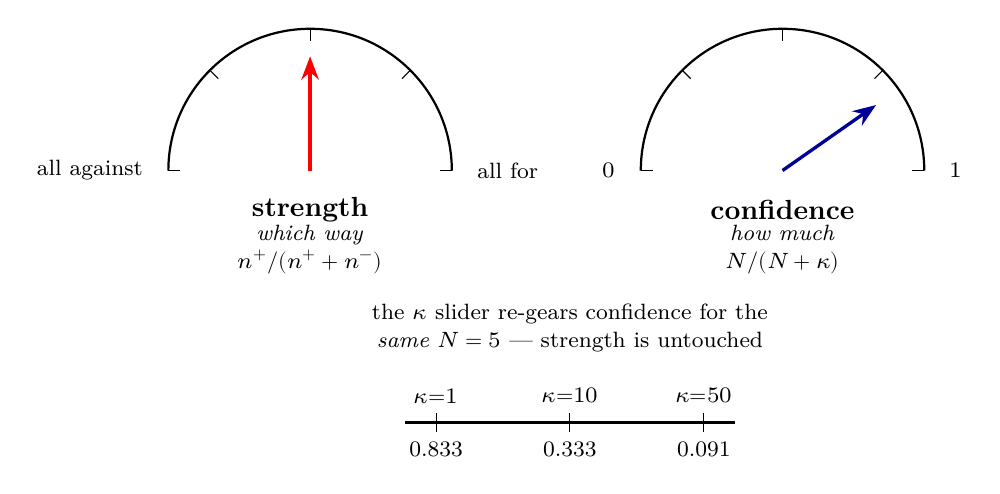
\begin{tikzpicture}[>=Stealth,scale=1.0]
  % ---- strength gauge ----
  \begin{scope}[shift={(0,0)}]
    \draw[thick] (0,0) arc (180:0:1.8);
    \foreach \a in {180,135,90,45,0} \draw ([shift={(1.8,0)}]\a:1.8)--([shift={(1.8,0)}]\a:1.65);
    \node[anchor=east] at (-0.2,0) {\footnotesize all against};
    \node[anchor=west] at (3.8,0) {\footnotesize all for};
    % needle at 0.5 -> straight up
    \draw[red,very thick,->] (1.8,0) -- ($(1.8,0)+(90:1.45)$);
    \node at (1.8,-0.5) {\textbf{strength}};
    \node[align=center] at (1.8,-1.0) {\footnotesize\emph{which way}\\[-2pt]\footnotesize $n^+/(n^++n^-)$};
  \end{scope}
  % ---- confidence gauge ----
  \begin{scope}[shift={(6,0)}]
    \draw[thick] (0,0) arc (180:0:1.8);
    \foreach \a in {180,135,90,45,0} \draw ([shift={(1.8,0)}]\a:1.8)--([shift={(1.8,0)}]\a:1.65);
    \node[anchor=east] at (-0.2,0) {\footnotesize $0$};
    \node[anchor=west] at (3.8,0) {\footnotesize $1$};
    \draw[blue!60!black,very thick,->] (1.8,0) -- ($(1.8,0)+(35:1.45)$);
    \node at (1.8,-0.5) {\textbf{confidence}};
    \node[align=center] at (1.8,-1.0) {\footnotesize\emph{how much}\\[-2pt]\footnotesize $N/(N+\kappa)$};
  \end{scope}
  % ---- kappa slider ----
  \begin{scope}[shift={(3.0,-3.2)}]
    \draw[thick] (0,0) -- (4.2,0);
    \foreach \x/\l/\v in {0.4/{$\kappa{=}1$}/{0.833}, 2.1/{$\kappa{=}10$}/{0.333}, 3.8/{$\kappa{=}50$}/{0.091}}{
      \draw (\x,0.12)--(\x,-0.12);
      \node[above] at (\x,0.12) {\footnotesize \l};
      \node[below] at (\x,-0.12) {\footnotesize \v};
    }
    \node[align=center] at (2.1,1.2) {\footnotesize the $\kappa$ slider re-gears confidence for the\\[-2pt]\footnotesize \emph{same} $N=5$ --- strength is untouched};
  \end{scope}
\end{tikzpicture}%
}
\vspace{0.7em}
\caption{Two dials. Strength reads which way the evidence leans (the ratio);
confidence reads how much evidence there is (the total), geared by the
calibration constant $\kappa$. The two move independently --- which is why one
number cannot do the job of both.}
\label{fig:dials}
\end{figure}

\section{Behind the dials: a set of admissible probabilities}\label{sec:spread}

We can say what the dials are really reading. Suppose your belief is about some
quantity --- ``the coin lands heads,'' or more generally the expected value of
some measurement $X$. If you knew the exact probability distribution of the
world, $X$ would have one exact expected value. But usually you do \emph{not}
know the exact distribution; you know a \emph{set} of distributions that are all
consistent with what you have seen. That set is the object behind the two
numbers. In the literature it is called a \textbf{credal set}; we will also just
call it the \emph{spread} of admissible probabilities.

\begin{quote}
\textbf{The whole content of $\STV{s}{c}$.}\footnote{The read-off:
\lid{lowerEnvelope} and \lid{upperEnvelope} in
\lpath{Mettapedia/ProbabilityTheory/ImpreciseProbability/ProjectiveCredal.lean};
see Appendix~\ref{app:formal}.} Take the spread. Ask your question
$X$. Each admissible distribution in the spread assigns $X$ some expected value;
sweeping over the spread, those values range between two endpoints, $L$ the
smallest expected value anyone in the spread allows and $U$ the largest. (For
the convex spreads we care about they fill the whole interval $[L,U]$; but only
the two endpoints are ever read off.) Then
\[
\begin{aligned}
  s &= \tfrac12(L+U) && \text{(the centre of the interval)},\\
  c &= g(U-L) && \text{(a decreasing function of its width)}.
\end{aligned}
\]
with $g(0)=1$ (zero width: full confidence) and $g$ falling toward $0$ as the
interval widens (maximum width: no confidence).
\end{quote}

That is the entire ``confidence characterization'' in one box, and the rest of
the paper is unpacking it. The endpoints $L$ and $U$ are the smallest and
largest honest answers; strength sits in the middle, and confidence asks how far
apart they are (Figure~\ref{fig:compress}).

\paragraph{This is the same confidence as Section~\ref{sec:dials}.} It is not a
second, competing definition. Take $g$ to be one-minus-width (the natural
``width-complement'' convention; Section~\ref{sec:zoo}, entry~5). After $N$
observations, the range of biases still consistent with the data has width
$\kappa/(N+\kappa)$, so $1-\text{width}=N/(N+\kappa)$ --- exactly the confidence
dial of Section~\ref{sec:dials}. The count rule $c=N/(N+\kappa)$ and the
envelope-width rule $c=g(U-L)$ are one belief seen two ways: counting evidence
\emph{is} narrowing the spread.

\paragraph{The coin, concretely.} Suppose all you know is that the coin's bias
$p$ lies somewhere in $[0.4,0.6]$. The spread is the family of coins with those
biases. The expected value of ``heads'' is just $p$, so it ranges over
$[0.4,0.6]$: here $L=0.4$, $U=0.6$. Strength $=\tfrac12(0.4+0.6)=0.5$;
confidence $=1-0.2=0.8$ (reading $g$ as one-minus-width). Now suppose you learn
nothing and
your spread is all of $[0,1]$: then $[L,U]=[0,1]$, width $1$, and confidence
drops to $0$ --- you have a centre ($0.5$) but no reason to trust it. Shrink the
spread to the single bias $\{0.5\}$ and the interval collapses to the point
$0.5$, width $0$, confidence $1$.

\paragraph{Why a set, and why two numbers lose information.} The spread is
richer than any two numbers: it can have a complicated shape, and it can pin
some questions while leaving others wide open. Recording only the centre and
width of one question's interval throws the rest away. That lost information is
not a bug --- it is the price of a compact, composable truth value --- but it is
exactly the source of the ``degrees of freedom'' this paper is about
(Figure~\ref{fig:compress}, grey box).

\begin{figure}[ht]
\centering
\resizebox{\textwidth}{!}{%
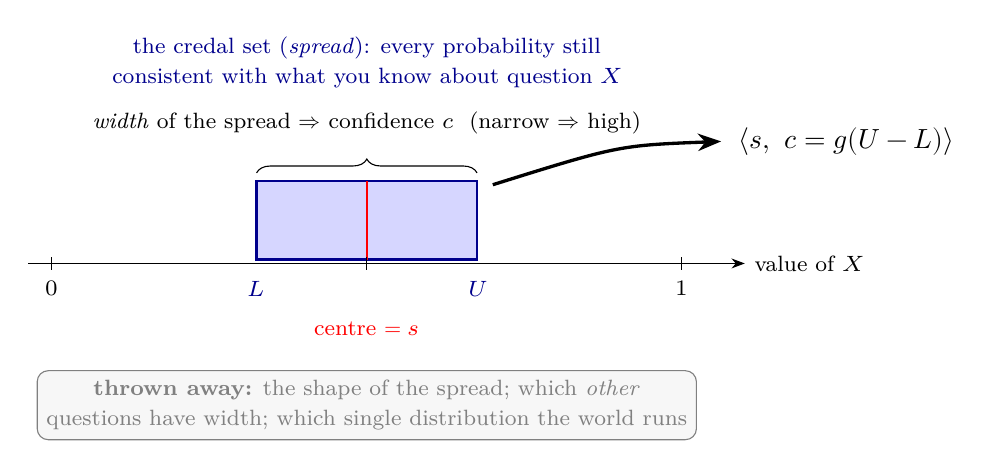
\begin{tikzpicture}[>=Stealth]
  % --- title for the spread (top, clearly separated) ---
  \node[blue!55!black,align=center] at (4,2.55)
       {\footnotesize the credal set (\emph{spread}): every probability still\\[-1pt]
        \footnotesize consistent with what you know about question $X$};
  % --- width brace + its label, just above the band ---
  \draw[decorate,decoration={brace,amplitude=5pt}] (2.6,1.15)--(5.4,1.15);
  \node[align=center] at (4,1.78)
       {\footnotesize \emph{width} of the spread $\Rightarrow$ confidence $c$ \ (narrow $\Rightarrow$ high)};
  % --- the spread band over [L,U] ---
  \fill[blue!16] (2.6,0.05) rectangle (5.4,1.05);
  \draw[blue!55!black,thick] (2.6,0.05) rectangle (5.4,1.05);
  % centre line -> strength
  \draw[red,thick] (4,0.05)--(4,1.05);
  % --- probability axis ---
  \draw[->] (-0.3,0) -- (8.8,0) node[right]{\footnotesize value of $X$};
  \foreach \x in {0,4,8} \draw (\x,0.08)--(\x,-0.08);
  \node[below] at (0,-0.1) {\footnotesize $0$};
  \node[below] at (8,-0.1) {\footnotesize $1$};
  \node[blue!55!black,below] at (2.6,-0.1) {\footnotesize $L$};
  \node[blue!55!black,below] at (5.4,-0.1) {\footnotesize $U$};
  \node[red,below] at (4,-0.62) {\footnotesize centre $=s$};
  % --- arrow to the compressed pair (upper right, clear of the axis) ---
  \draw[->,very thick] (5.6,1.0) .. controls (7.2,1.5) .. (8.5,1.55);
  \node[anchor=west] at (8.6,1.55) {$\STV{s}{\,c=g(U-L)}$};
  % --- what's lost (below everything, clear of the axis labels) ---
  \node[draw,gray,rounded corners,align=center,text=gray,fill=gray!6] at (4,-1.8)
    {\footnotesize \textbf{thrown away:} the shape of the spread; which \emph{other}\\[-1pt]
     \footnotesize questions have width; which single distribution the world runs};
\end{tikzpicture}%
}
\caption{Compression. The two numbers are a lossy photo of a whole set: strength
is the centre of the interval the set allows for your question, confidence falls
with its width. Everything in the grey box is invisible to $\STV{s}{c}$.}
\label{fig:compress}
\end{figure}

\section{The fork in the road: pinned, or a range}\label{sec:fork}

Everything above leads to one clean dichotomy, and it is the technical heart of
the paper. Fix a spread and a question $X$. Exactly one of two things happens.

\begin{itemize}
\item \textbf{Pinned.} Every admissible distribution in the spread assigns $X$
the \emph{same} expected value. Then $L=U$: the interval is a single point, the
width is zero, and confidence sits at its ceiling. The two numbers tell the
whole story --- there is nothing else to know about $X$.
\item \textbf{A genuine range.} Two admissible distributions \emph{disagree}
about $X$. Then $L<U$: the interval has real width, strength is its midpoint,
and confidence is honestly below the ceiling. The two numbers report the range,
not a single value.
\end{itemize}

These are the only two cases, and they are mutually exclusive: a question cannot
be both pinned and have width (Figure~\ref{fig:fork}). This is stated formally,
and machine-checked, in Appendix~\ref{app:formal}\footnote{Lean:
\lid{credalSetDetermines} and \lid{credalSetHasStrictWidth} (with the collapse,
width, and mutual-exclusion theorems) in
\lpath{Mettapedia/ProbabilityTheory/ImpreciseProbability/ProjectiveCredal.lean};
see Appendix~\ref{app:formal}, item~\ref{item:dich}.} (the \emph{pinned/range
dichotomy} and its mutual exclusion).

\paragraph{A ``pinned'' example.} If the spread is a single
distribution, \emph{everything} is pinned: every question has $L=U$, every
confidence is at the ceiling. There is no freedom anywhere --- the belief is as
sharp as belief can be.

\paragraph{A ``range'' example: two stuck magnets.} Imagine two coupled
sites that must agree: either both ``up'' or both ``down,'' and you do not know
which world you are in. The spread is the two distributions \{all-up\},
\{all-down\}. Ask: \emph{is the first site up?} In the all-up world the answer is
$1$; in the all-down world it is $0$. So the interval is $[0,1]$, width $1$,
confidence $0$: maximally uncertain, even though each individual world is itself
perfectly definite. The uncertainty is not noise inside a world --- it is not
knowing which world.\footnote{The two-magnets witness:
\lid{twoSpinMagnetEnvelope\_nontrivial} in
\lpath{Mettapedia/ProbabilityTheory/ImpreciseProbability/ProjectiveCredal.lean};
see Appendix~\ref{app:formal}, item~\ref{item:strong}.}

\begin{figure}[ht]
\centering
\resizebox{\textwidth}{!}{%
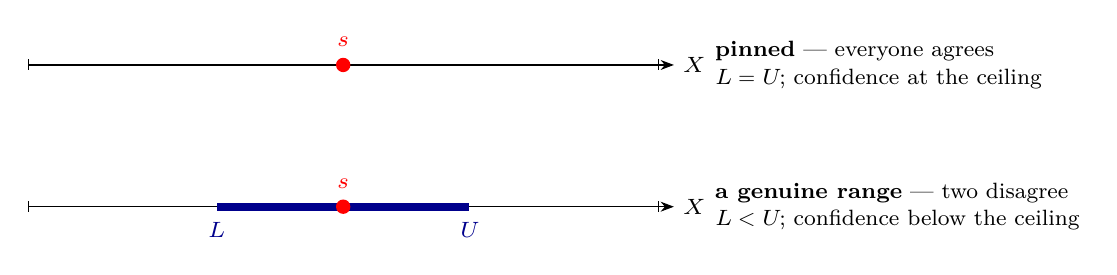
\begin{tikzpicture}[>=Stealth]
  % top line: determined
  \begin{scope}[shift={(0,1.4)}]
    \draw[->] (0,0)--(8.2,0) node[right]{\footnotesize $X$};
    \foreach \x in {0,4,8} \draw (\x,0.07)--(\x,-0.07);
    \fill[red] (4,0) circle (2.6pt);
    \node[red,above=3pt] at (4,0) {\footnotesize $s$};
    \node[align=left,anchor=west] at (8.6,0)
      {\footnotesize \textbf{pinned} --- everyone agrees\\[-2pt]
       \footnotesize $L=U$; confidence at the ceiling};
  \end{scope}
  % bottom line: interval
  \begin{scope}[shift={(0,-0.4)}]
    \draw[->] (0,0)--(8.2,0) node[right]{\footnotesize $X$};
    \foreach \x in {0,4,8} \draw (\x,0.07)--(\x,-0.07);
    \draw[blue!55!black,line width=3pt] (2.4,0)--(5.6,0);
    \fill[red] (4,0) circle (2.6pt);
    \node[blue!55!black,below=2pt] at (2.4,0) {\footnotesize $L$};
    \node[blue!55!black,below=2pt] at (5.6,0) {\footnotesize $U$};
    \node[red,above=3pt] at (4,0) {\footnotesize $s$};
    \node[align=left,anchor=west] at (8.6,0)
      {\footnotesize \textbf{a genuine range} --- two disagree\\[-2pt]
       \footnotesize $L<U$; confidence below the ceiling};
  \end{scope}
\end{tikzpicture}%
}
\caption{The fork. For any question of any spread: either every admissible
distribution agrees (a single pinned value, top) or two disagree (a genuine
interval, bottom). This same picture returns for the infinite cases in
Section~\ref{sec:infinite}: weak coupling lands on top, strong coupling on the
bottom. ($s$ is drawn at the midpoint convention.)}
\label{fig:fork}
\end{figure}

\section{Building a big belief from small pieces}\label{sec:build}

So far the spread was small enough to picture. For a large or infinite world ---
say, a belief about a whole grid of interacting variables --- you cannot write
the spread down directly. Instead you specify it \emph{locally}: you say what is
admissible on each small ``window'' of the world, and you glue the windows
together consistently. The global spread is then everything that fits all the
local pieces at once.

You do not need the machinery to feel the two extremes:

\begin{itemize}
\item \textbf{Tightest possible.} If each local piece allows exactly one
distribution, the glued global spread is a single distribution: everything is
pinned, no freedom (Section~\ref{sec:fork}, ``pinned'').
\item \textbf{Loosest possible.} If each local piece allows \emph{everything},
the global spread contains every distribution: almost every question has full
width, maximum freedom.
\end{itemize}

Real models live between these. The interesting content is: \emph{where} does
freedom enter as you build up, and which kinds can the two-number summary see?
That is the next section. (The formal construction --- local windows, restriction
maps, the glued limit --- is Appendix~\ref{app:formal}, items \ref{item:global}
and following; the body needs only ``specify locally, glue globally.'')

\section{Three places freedom can hide}\label{sec:three}

Pulling it together, the wiggle room behind $\STV{s}{c}$ comes from three
sources (Figure~\ref{fig:three}).

\begin{description}
\item[(A) The modeller's freedom.] \emph{How wide you chose to make the local
pieces.} If you declare a quantity known only to within $[0.4,0.6]$, you put
that width there on purpose. The two numbers report it faithfully: this freedom
is \textbf{visible}.
\item[(B) The world's freedom.] \emph{Which single true distribution the world
actually runs, inside your spread.} Your spread might allow many; the world picks
one. The pair $\STV{s}{c}$ cannot see which --- and that is correct, because the
belief is a statement about the whole spread, not a guess at the world's secret
pick. This freedom is \textbf{invisible}, by design. (It is the kind of
uncertainty that more local data does not remove: it is about which possibility
is real, not about a fuzzy measurement.) A truth value that \emph{changed} with
the world's hidden pick would be claiming knowledge it cannot have from the
evidence --- so its blindness here is soundness, not a defect.
\item[(C) The structure's own freedom.] \emph{When gluing infinitely many local
pieces admits several global solutions to the very same local rules.} No
modeller put it there; no single ``true world inside the spread'' explains it
away. It is produced by the structure itself, and the two numbers \emph{can} see
it (it shows up as genuine width). This is the surprise of the infinite case
(Section~\ref{sec:infinite}).
\end{description}

\begin{observation}[the thesis in one line]
$\STV{s}{c}$ is a property of the whole spread, not of any single distribution in
it. So it sees how wide you made the model \textup{(A)} and whether the structure
forces a range \textup{(C)}, but it is --- correctly --- blind to which member
the world actually picked \textup{(B)}.
\end{observation}

\begin{figure}[ht]
\centering
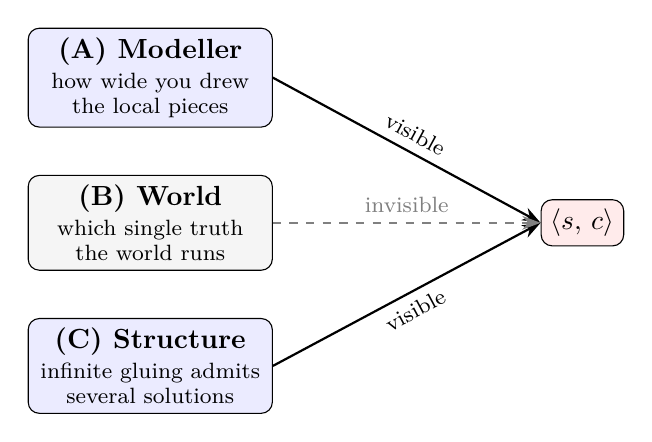
\begin{tikzpicture}[>=Stealth,node distance=6mm]
  \node[draw,rounded corners,fill=blue!8,align=center,minimum width=3.1cm] (A)
    {\textbf{(A) Modeller}\\[-1pt]\footnotesize how wide you drew\\[-3pt]\footnotesize the local pieces};
  \node[draw,rounded corners,fill=gray!8,align=center,minimum width=3.1cm,below=of A] (B)
    {\textbf{(B) World}\\[-1pt]\footnotesize which single truth\\[-3pt]\footnotesize the world runs};
  \node[draw,rounded corners,fill=blue!8,align=center,minimum width=3.1cm,below=of B] (C)
    {\textbf{(C) Structure}\\[-1pt]\footnotesize infinite gluing admits\\[-3pt]\footnotesize several solutions};
  \node[draw,rounded corners,fill=red!8,align=center,right=34mm of B] (S)
    {$\STV{s}{c}$};
  \draw[->,thick] (A.east) -- (S.west) node[midway,above,sloped]{\footnotesize visible};
  \draw[->,thick] (C.east) -- (S.west) node[midway,below,sloped]{\footnotesize visible};
  \draw[->,gray,dashed,thick] (B.east) -- (S.west) node[midway,above]{\footnotesize invisible};
\end{tikzpicture}
\caption{Three sources of freedom and what the two numbers can see. (A) and (C)
reach $\STV{s}{c}$; (B), the world's single hidden pick, does not --- and that
blindness is the correct behaviour, because the truth value describes the set,
not the pick. (A) is freedom you \emph{declared}; (C) is freedom the structure
produces \emph{emergently} --- different origins, both visible.}
\label{fig:three}
\end{figure}

\section{Three infinite stories}\label{sec:infinite}

The same fork --- pinned or a range --- recurs when the world is infinite, and
this is where it gets genuinely interesting. We tell three stories in plain
language; the theorems behind them are in Appendix~\ref{app:formal}.

\subsection{When do snapshots add up to a movie? (order-free streams)}
\label{sec:exch}

You watch a stream where only the \emph{counts} matter, not the order ---
patient responses, defects coming off a line, fraud flags. ``Order does not
matter'' is a real assumption with a famous name (\emph{exchangeability}), and a
beautiful classical fact (de Finetti's theorem~\cite{definetti37}) says such a
stream behaves exactly like repeatedly flipping a coin of \emph{unknown} bias,
averaged over your uncertainty about the bias.

From any finite prefix you can always write down a sensible next-step forecast.
The textbook one is Laplace's rule: $3$ successes in $5$ predicts
$\tfrac{3+1}{5+2}=0.5714$ for the next; $30$ in $50$ predicts $0.5962$. That
forecast is \emph{always available}. The subtle part is the stronger claim that
your finite forecasts knit together into \emph{one} consistent infinite law that
answers \emph{every} question coherently. That stronger claim is not automatic:
it holds exactly at a precise compatibility boundary (Appendix~\ref{app:formal},
item~\ref{item:exch}).\footnote{Lean: the \emph{sharp compatibility} crown (and
its refuted ``every component degenerate'' tightening) in
\lpath{Mettapedia/Logic/DeFinettiProjectiveCredalBridge.lean}; full name and
statement in Appendix~\ref{app:formal}, item~\ref{item:exch}.}

\begin{quote}
\textbf{Takeaway.} Having a forecast for tomorrow is free; having a coherent
theory of the whole future is not --- and we pin down exactly where the line is.
A caution that survives the formalization: it is tempting to require the unknown
bias to be pinned to an exact value (always $0$ or always $1$, never in between),
but that would forbid the honest ``I'm not sure of the bias'' case --- which is
the whole reason to carry a set of coins instead of one. The real boundary is
more permissive than that.
\end{quote}

\subsection{Weak coupling: one precise answer}\label{sec:weak}

Now picture not one variable but a vast grid of them --- sensors, pixels,
people --- where each one only \emph{nudges} its neighbours a little. ``A little''
can be made into a budget you check by adding up the nudges.

\begin{quote}
\textbf{The result.} When every local influence is small enough (the budget
holds), the infinite system has \emph{exactly one} global behaviour consistent
with the local rules. Every finite question then gets one precise answer:
strength is a single point, confidence sits at the ceiling. Distant conditions
wash out --- what you fix far away cannot reach the centre. This lands on the
\emph{top} of the fork in Figure~\ref{fig:fork}.
\end{quote}

Intuitively: if nothing pushes hard, faraway stuff does not matter, so the two
numbers tell the whole story. (This is the de-jargoned form of the classical
Dobrushin uniqueness condition~\cite{dobrushin68}; Appendix~\ref{app:formal},
item~\ref{item:weak}.\footnote{Lean: \lid{dlrQueryDetermined\_of\_uniform} (with
the precise-envelope and global-uniqueness theorems) in
\lpath{Mettapedia/Logic/MarkovLogicInfiniteCredalBridge.lean}.} We prove this
direction; we do \emph{not} claim the
converse, that failing the budget forces a range.)

\subsection{Strong coupling: a genuine interval the distant edges control}
\label{sec:strong}

Same grid, opposite regime: now neighbours pull \emph{hard} to agree --- a magnet
near freezing, a spreading contagion, an image whose adjacent pixels strongly
match.

\begin{quote}
\textbf{The result.} Now the infinite system has \emph{more than one} global
behaviour consistent with the same local rules, and --- the striking part ---
\emph{what you fix at the far-away boundary changes the answer in the centre}. A
question at the middle gets a \emph{genuine interval}, not a point: confidence is
honestly below the ceiling, and that width is not ignorance you could erase with
more local data. It is the system's own structure. This lands on the
\emph{bottom} of the fork.
\end{quote}

This is the same setup as Section~\ref{sec:weak} at a different coupling
strength: \emph{weak coupling gives a point, strong coupling gives an interval.}
That single contrast is the whole infinite story. Why does the far-away boundary
reach the centre at all? Because flipping it would force a long ring of
neighbours to disagree, and long rings of disagreement are exponentially
unlikely when the coupling is strong --- so the centre keeps a memory of the edge
that no amount of interior data can erase. The strong-coupling side is the
hardest theorem in the project --- it is a low-temperature two-dimensional magnet
whose centre genuinely depends on the boundary --- and it is stated, with the one
machine-checked guarantee it provides, in Appendix~\ref{app:formal},
item~\ref{item:strong}.\footnote{Lean: the symmetric-grid strict-interval crown,
proved unconditionally, in
\lpath{Mettapedia/Logic/MarkovLogicInfiniteSymmetricGridExample.lean}; full name
and statement in Appendix~\ref{app:formal}, item~\ref{item:strong}.} (For the connoisseur: the underlying tool is a Peierls
contour argument; we do not need it here, and nothing in this section depends on
the proof technique.)

\section{The knob zoo: nineteen places two numbers can fool you}\label{sec:zoo}

This is the practical payoff, and the part to keep open while you work. Each
entry is a \emph{degree of freedom}: a modelling choice under which two beliefs
can share the same $\STV{s}{c}$ yet mean different things, or under which a single
``obvious'' default silently commits you to something. Each comes as: the idea in
a sentence, the smallest number that shows it, and the trap it prevents. Every
number here is reproduced by the runnable pack (Appendix~\ref{app:run}); every
entry names its formal anchor in Appendix~\ref{app:formal}.\footnote{The new
canaries for DoF 8, 11, and 18 are in
\lpath{Mettapedia/Logic/PLNConfidenceDoFCanary.lean};
\lpath{papers/pln-confidence-examples/lean/DOF-LEAN-MAP.md} maps every degree of
freedom to its theorem.}

\begin{enumerate}
\item \textbf{Evidence scale $\kappa$.}\footnote{Lean:
\lid{walley\_width\_complement\_forces\_plnOdds} forces the odds shape while
leaving $\kappa$ free (\lpath{Mettapedia/Logic/PLNConfidenceWeight.lean});
strength is \lid{posteriorMeanStrength} (\lpath{Mettapedia/Logic/PLNTruthTower.lean}).}
How much evidence counts as ``a lot'' is
a domain choice. The same $N=5$ gives confidence $0.833/0.333/0.091$ at
$\kappa=1/10/50$. \emph{Trap:} fixing $\kappa=1$ everywhere lets a lone weak hit
claim $0.83$ confidence it never earned.

\knobpic{%
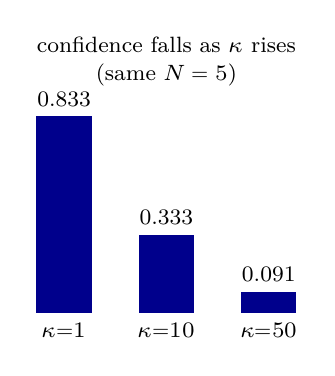
\begin{tikzpicture}
  \foreach \x/\h/\k/\v in {0/2.5/1/0.833, 1.3/1.0/10/0.333, 2.6/0.27/50/0.091}{
    \fill[blue!55!black] (\x,0) rectangle ({\x+0.7},\h);
    \node[below] at ({\x+0.35},0) {\footnotesize $\kappa{=}\k$};
    \node[above] at ({\x+0.35},\h) {\footnotesize \v};
  }
  \node[align=center] at (1.65,3.2) {\footnotesize confidence falls as $\kappa$ rises\\[-2pt]\footnotesize (same $N=5$)};
\end{tikzpicture}}

\item \textbf{Prior context for strength.}\footnote{Lean:
\lid{posteriorMeanStrength\_improper\_eq\_mle} in
\lpath{Mettapedia/Logic/PLNTruthTower.lean}.} The same counts read differently
under maximum-likelihood, a uniform prior, or Jeffreys'. From a single positive
$(1,0)$: MLE $1.0$, uniform-prior mean $0.667$, Jeffreys $0.75$ --- and all
converge to $\approx0.999$ once $1000$ observations pile up. \emph{Trap:}
pretending strength is context-free silently bakes in a prior.

\knobpic{%
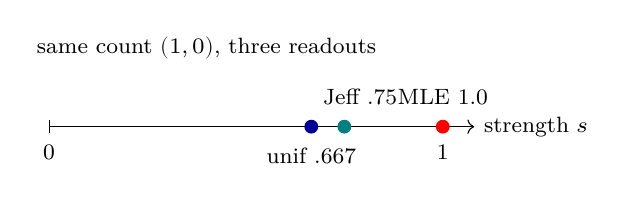
\begin{tikzpicture}
  \draw[->](0,0)--(5.4,0) node[right]{\footnotesize strength $s$};
  \draw(0,0.08)--(0,-0.08); \draw(5,0.08)--(5,-0.08);
  \node[below] at (0,-0.1){\footnotesize 0}; \node[below] at (5,-0.1){\footnotesize 1};
  \fill[blue!60!black](3.33,0)circle(2.5pt); \node[below] at (3.33,-0.15){\footnotesize unif .667};
  \fill[teal](3.75,0)circle(2.5pt); \node[above] at (3.95,0.15){\footnotesize Jeff .75};
  \fill[red](5,0)circle(2.5pt); \node[above] at (5,0.15){\footnotesize MLE 1.0};
  \node at (2.0,1.0){\footnotesize same count $(1,0)$, three readouts};
\end{tikzpicture}}

\item \textbf{Total versus ratio.}\footnote{Lean:
\lid{strength\_mem\_unit\_of\_total\_ne\_zero} in
\lpath{Mettapedia/Logic/PLNTruthTower.lean}.} Strength reads the ratio, confidence the
total --- the reason there are two numbers at all. $1/1,10/10,100/100$ all have
strength $0.5$ with confidence $0.667/0.952/0.995$; $1/1$ versus $2/0$ share the
total (confidence $0.667$) but split on strength ($0.5$ vs $1.0$). \emph{Trap:}
any one-number truth value equates $1/1$ with $100/100$.

\knobpic{%
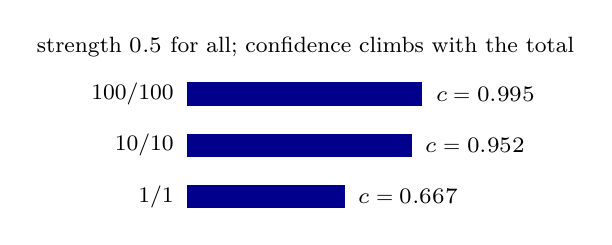
\begin{tikzpicture}
  \foreach \y/\n/\v in {0/{1/1}/0.667, 0.65/{10/10}/0.952, 1.3/{100/100}/0.995}{
    \node[left] at (-0.05,{\y+0.15}){\footnotesize \n};
    \fill[blue!55!black](0,\y) rectangle ({3*\v},{\y+0.3});
    \node[right] at ({3*\v+0.05},{\y+0.15}){\footnotesize $c={\v}$};
  }
  \node at (1.5,2.05){\footnotesize strength $0.5$ for all; confidence climbs with the total};
\end{tikzpicture}}

\item \textbf{Confidence chart.}\footnote{Lean:
\lid{reserveHalfCoordinate\_not\_walley\_width\_complement} (a chart that
reconstructs evidence yet is not the odds chart) in
\lpath{Mettapedia/Logic/PLNConfidenceWeight.lean}.} Recovering the evidence count needs only
\emph{some} invertible scale; it does not force PLN's particular one. The same
recovered evidence displayed three ways gives $0.833$ (PLN odds), $0.455$
(a reserve-half chart), $0.874$ (an arctangent chart). \emph{Trap:} combining
evidence in a display chart instead of in evidence-count space.

\knobpic{%
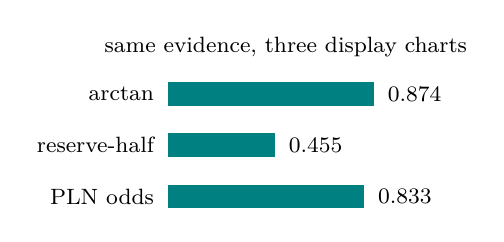
\begin{tikzpicture}
  \foreach \y/\n/\v in {0/{PLN odds}/0.833, 0.65/{reserve-half}/0.455, 1.3/{arctan}/0.874}{
    \node[left] at (-0.05,{\y+0.15}){\footnotesize \n};
    \fill[teal](0,\y) rectangle ({3*\v},{\y+0.3});
    \node[right] at ({3*\v+0.05},{\y+0.15}){\footnotesize \v};
  }
  \node at (1.5,2.05){\footnotesize same evidence, three display charts};
\end{tikzpicture}}

\item \textbf{Width-complement convention.}\footnote{Lean:
\lid{WidthComplementCompatible} (\lpath{Mettapedia/Logic/PLNTruthTower.lean})
and \lid{walley\_width\_complement\_forces\_plnOdds}
(\lpath{Mettapedia/Logic/PLNConfidenceWeight.lean}).} Setting confidence $=1-\text{width}$
is natural but still a convention, and it needs a scale. A binary interval gives
$0.4$; a bounded utility, correctly range-normalized, also $0.4$; the same
utility left un-normalized gives the deliberate nonsense $-59.0$. \emph{Trap:}
applying width-complement to dollar-valued gambles without normalizing.

\knobpic{%
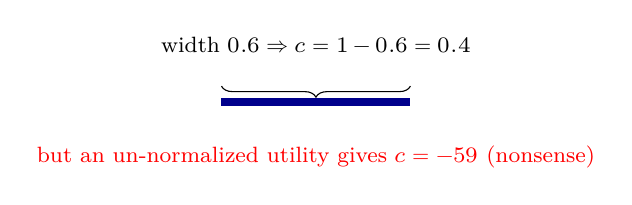
\begin{tikzpicture}
  \draw[blue!55!black,line width=3pt](0.6,0)--(3.0,0);
  \draw[decorate,decoration={brace,amplitude=4pt}](3.0,0.2)--(0.6,0.2);
  \node[above] at (1.8,0.5){\footnotesize width $0.6\Rightarrow c=1-0.6=0.4$};
  \node[red] at (1.8,-0.7){\footnotesize but an un-normalized utility gives $c=-59$ (nonsense)};
\end{tikzpicture}}

\item \textbf{Interval point selector.}\footnote{Lean:
\lid{generic\_itv\_does\_not\_force\_point\_projection} in
\lpath{Mettapedia/Logic/PLNTruthTheoryIndex.lean}.} A real interval $[L,U]$ does not pick its
own display point. Lower / midpoint / upper on one interval: $0.2/0.5/0.8$.
\emph{Trap:} a safety decision shown the midpoint when it needed the lower bound.

\knobpic{%
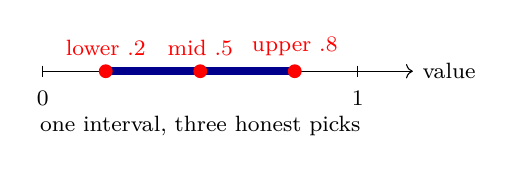
\begin{tikzpicture}
  \draw[->](0,0)--(4.7,0) node[right]{\footnotesize value};
  \draw(0,0.07)--(0,-0.07);\draw(4,0.07)--(4,-0.07);
  \node[below] at(0,-0.12){\footnotesize 0};\node[below] at(4,-0.12){\footnotesize 1};
  \draw[blue!55!black,line width=3pt](0.8,0)--(3.2,0);
  \fill[red](0.8,0)circle(2.5pt) node[above=2pt]{\footnotesize lower .2};
  \fill[red](2.0,0)circle(2.5pt) node[above=2pt]{\footnotesize mid .5};
  \fill[red](3.2,0)circle(2.5pt) node[above=2pt]{\footnotesize upper .8};
  \node at (2,-0.7){\footnotesize one interval, three honest picks};
\end{tikzpicture}}

\item \textbf{Credal shape beyond one interval.}\footnote{Lean:
\lid{CredalProjectionTower} in \lpath{Mettapedia/Logic/PLNTruthTower.lean}.} Two spreads can agree on one
question and disagree on another --- the very reason $\STV{s}{c}$ is a
compression. Two joint models with identical marginals $P(A)=P(B)=0.5$ can have
conjunction $0.5$ (perfectly dependent) or $0.0$ (mutually exclusive); the whole
range $[0,0.5]$ is invisible to the marginal summary. \emph{Trap:} certifying two
incompatible joint models ``the same'' because their margins match.

\knobpic{%
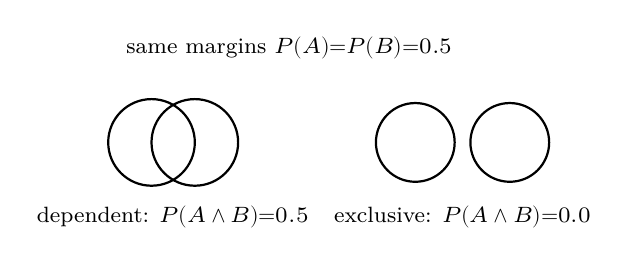
\begin{tikzpicture}
  \begin{scope}
    \draw[thick] (0,0) circle (0.55); \draw[thick] (0.55,0) circle (0.55);
    \node at (0.27,-0.95){\footnotesize dependent: $P(A\wedge B){=}0.5$};
  \end{scope}
  \begin{scope}[shift={(3.4,0)}]
    \draw[thick] (-0.05,0) circle (0.5); \draw[thick] (1.15,0) circle (0.5);
    \node at (0.55,-0.95){\footnotesize exclusive: $P(A\wedge B){=}0.0$};
  \end{scope}
  \node at (1.75,1.2){\footnotesize same margins $P(A){=}P(B){=}0.5$};
\end{tikzpicture}}

\item \textbf{Which uncertainty method (the ``backend'').}\footnote{Lean:
\lid{beta\_mean\_strictly\_inside\_walley\_idm\_interval} in
\lpath{Mettapedia/Logic/PLNConfidenceDoFCanary.lean}; see Appendix~\ref{app:formal}.} Feed the \emph{same}
data to two different uncertainty methods and you get answers of different
\emph{shape}. From $2$ ``yes'' and $3$ ``no'': a single-distribution Bayesian
method returns one best number (the Beta posterior mean $\tfrac{3}{7}\approx
0.429$), while a cautious \emph{imprecise} method returns a whole interval of
defensible values, $[\tfrac{2}{7},\tfrac{4}{7}]=[0.286,0.571]$. The Bayesian
point lands inside that interval --- it simply declines to show the range.
\emph{Trap:} collapsing the cautious interval down to the single point ``for
convenience,'' silently discarding the safety margin.

\knobpic{%
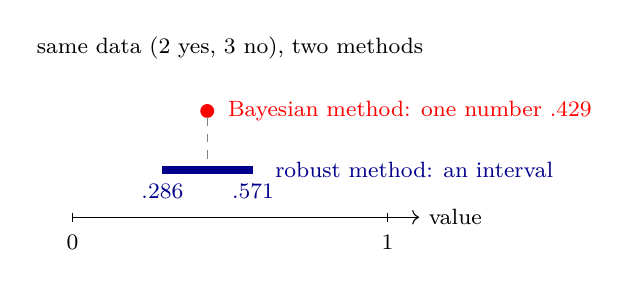
\begin{tikzpicture}
  \draw[->](0,0)--(4.4,0) node[right]{\footnotesize value};
  \draw(0,0.06)--(0,-0.06);\draw(4,0.06)--(4,-0.06);
  \node[below] at(0,-0.1){\footnotesize 0};\node[below] at(4,-0.1){\footnotesize 1};
  \draw[blue!55!black,line width=3pt](1.14,0.6)--(2.29,0.6);
  \node[blue!55!black,below] at(1.14,0.55){\footnotesize .286};
  \node[blue!55!black,below] at(2.29,0.55){\footnotesize .571};
  \node[blue!55!black,right] at(2.45,0.6){\footnotesize robust method: an interval};
  \fill[red](1.71,1.35)circle(2.5pt);
  \node[red,right] at(1.85,1.35){\footnotesize Bayesian method: one number .429};
  \draw[gray,dashed](1.71,1.27)--(1.71,0.66);
  \node at (2.0,2.15){\footnotesize same data (2 yes, 3 no), two methods};
\end{tikzpicture}}

\item \textbf{Credible level / tolerance.}\footnote{Lean:
\lid{walleyCategorical\_credibility\_eq} in
\lpath{Mettapedia/Logic/PLNTruthTower.lean}.} A Bayesian interval also carries a
chosen level ($90/95/99\%$) --- a different knob from $\kappa$. $\kappa$ governs
how evidence accumulates; the level governs what you \emph{ask} of a finished
posterior. \emph{Trap:} confusing ``more evidence'' with ``a tighter requested
interval.''

\knobpic{%
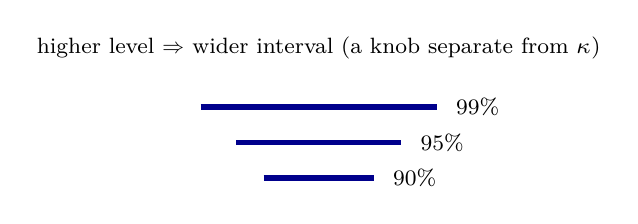
\begin{tikzpicture}
  \foreach \y/\w/\l in {0/0.7/90, 0.45/1.05/95, 0.9/1.5/99}{
    \draw[line width=2pt,blue!55!black] ({2-\w},\y)--({2+\w},\y);
    \node[right] at ({2+\w+0.12},\y){\footnotesize \l\%};
  }
  \node at (2,1.65){\footnotesize higher level $\Rightarrow$ wider interval (a knob separate from $\kappa$)};
\end{tikzpicture}}

\item \textbf{Categorical query.}\footnote{Lean:
\lid{categoricalSurface\_idmEnvelope\_forced\_by\_aggregate} in
\lpath{Mettapedia/Logic/PLNTruthTower.lean}.} In a multi-class model the total evidence is
shared but each category has its own confidence. In a $1000$-sample $3$-class
model: the common class has strength $0.90$, confidence $0.999$; a rare class has
strength $0.002$, confidence $0.167$ \emph{despite} the huge total. \emph{Trap:}
``the classifier is $99.9\%$ confident'' hiding that a class rests on two
observations.

\knobpic{%
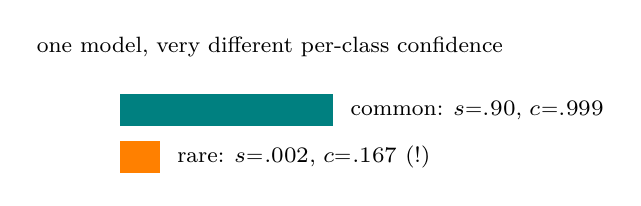
\begin{tikzpicture}
  \fill[teal] (0,0) rectangle (2.7,0.4);
  \node[right] at (2.8,0.2){\footnotesize common: $s{=}.90$, $c{=}.999$};
  \fill[orange] (0,-0.6) rectangle (0.5,-0.2);
  \node[right] at (0.6,-0.4){\footnotesize rare: $s{=}.002$, $c{=}.167$ (!)};
  \node at (1.9,1.0){\footnotesize one model, very different per-class confidence};
\end{tikzpicture}}

\item \textbf{Evidence discounting.}\footnote{Lean:
\lid{power\_discount\_scales\_logodds} in
\lpath{Mettapedia/Logic/PLNConfidenceDoFCanary.lean}.} Evidence can be reweighted for quality,
rarity, or route before it counts. Power-discounting scales the log-odds
linearly; discounted totals of $4.57,12,104$ give confidences
$0.821/0.923/0.991$. \emph{Trap:} treating correlated hits as independent and
overstating confidence.

\knobpic{%
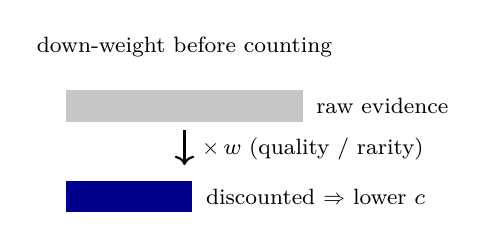
\begin{tikzpicture}
  \fill[gray!45](0,0.2) rectangle (3,0.6); \node[right] at(3.05,0.4){\footnotesize raw evidence};
  \draw[->,thick](1.5,0.1)--(1.5,-0.35);
  \node[right] at (1.6,-0.15){\footnotesize $\times\,w$ (quality / rarity)};
  \fill[blue!55!black](0,-0.95) rectangle (1.6,-0.55);
  \node[right] at(1.65,-0.75){\footnotesize discounted $\Rightarrow$ lower $c$};
  \node at (1.5,1.15){\footnotesize down-weight before counting};
\end{tikzpicture}}

\item \textbf{Local credal specification.}\footnote{Lean:
\lid{finiteLowerPrevision} and \lid{coherentDesirableSet} in
\lpath{Mettapedia/Logic/PLNTruthTower.lean}.} In a built-up model the modeller
chooses how wide each local piece is --- the intended-imprecision knob (source
(A) of Section~\ref{sec:three}). \emph{Trap:} hiding local ambiguity behind a
single precise prior, so later confidence looks unjustifiably high.

\knobpic{%
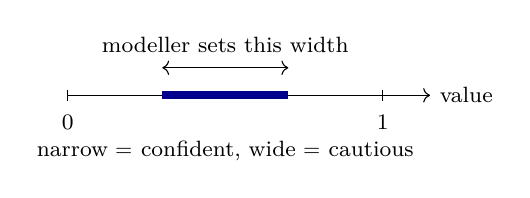
\begin{tikzpicture}
  \draw[->](0,0)--(4.6,0) node[right]{\footnotesize value};
  \draw(0,0.07)--(0,-0.07);\draw(4,0.07)--(4,-0.07);
  \node[below] at(0,-0.12){\footnotesize 0};\node[below] at(4,-0.12){\footnotesize 1};
  \draw[<->](1.2,0.35)--(2.8,0.35);
  \node[above] at(2,0.42){\footnotesize modeller sets this width};
  \draw[blue!55!black,line width=3pt](1.2,0)--(2.8,0);
  \node at (2,-0.7){\footnotesize narrow $=$ confident, wide $=$ cautious};
\end{tikzpicture}}

\item \textbf{Compatible completion.}\footnote{Lean: the sharp-compatibility
crown in \lpath{Mettapedia/Logic/DeFinettiProjectiveCredalBridge.lean}; see
Appendix~\ref{app:formal}, item~\ref{item:exch}.} Finite-prefix forecasts always exist; a
full infinite law does not always exist (Section~\ref{sec:exch}). The Laplace
readout $3/5\to0.5714$, $30/50\to0.5962$ is always available; the consistent
whole-process law is a separate boundary condition. \emph{Trap:} calling finite
forecasts a process law without the compatibility witness.

\knobpic{%
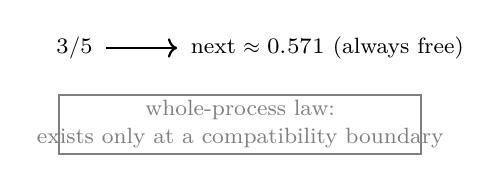
\begin{tikzpicture}
  \node at (0.2,0){\footnotesize $3/5$};
  \draw[->,thick](0.6,0)--(1.5,0);
  \node[right] at (1.55,0){\footnotesize next $\approx 0.571$ (always free)};
  \draw[gray,thick] (0.0,-1.35) rectangle (4.6,-0.6);
  \node[gray,align=center] at (2.3,-0.97){\footnotesize whole-process law:\\[-2pt]\footnotesize exists only at a compatibility boundary};
\end{tikzpicture}}

\item \textbf{Completion extreme point.}\footnote{Lean:
\lid{boundedMeasurableCredalSetHasStrictWidth} in
\lpath{Mettapedia/ProbabilityTheory/ImpreciseProbability/ProjectiveCredal.lean}.} Inside a fixed spread the world runs one
true distribution, and that single pick is invisible to $\STV{s}{c}$ --- correctly
(source (B)). The two stuck magnets witness it: two admissible worlds disagree,
so no single determined readout is justified. \emph{Trap:} an inference rule that
pretends to know which world is real.

\knobpic{%
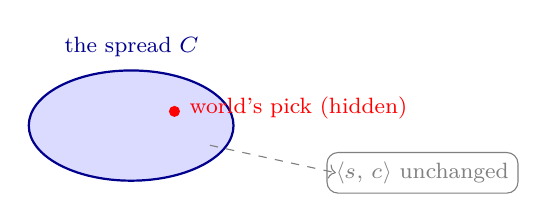
\begin{tikzpicture}
  \fill[blue!14](0,0) ellipse (1.3 and 0.7);
  \draw[blue!55!black,thick](0,0) ellipse (1.3 and 0.7);
  \node[blue!55!black] at (0,1.0){\footnotesize the spread $C$};
  \fill[red](0.55,0.18)circle(2pt);
  \node[red,right] at(0.62,0.22){\footnotesize world's pick (hidden)};
  \draw[->,dashed,gray](1.0,-0.25)--(2.6,-0.6);
  \node[draw,gray,rounded corners,text=gray] at (3.7,-0.6){\footnotesize $\STV{s}{c}$ unchanged};
\end{tikzpicture}}

\item \textbf{Phase transition / infinite boundary.}\footnote{Lean: the
weak-coupling collapse (\lpath{Mettapedia/Logic/MarkovLogicInfiniteCredalBridge.lean})
and the strong-coupling crown
(\lpath{Mettapedia/Logic/MarkovLogicInfiniteSymmetricGridExample.lean}); see
Appendix~\ref{app:formal}, items~\ref{item:weak} and~\ref{item:strong}.} Some infinite
specifications admit several global solutions to the same local rules (source
(C)). Weak coupling collapses the interval (Section~\ref{sec:weak}); strong
coupling keeps it open, controlled by distant boundaries
(Section~\ref{sec:strong}). \emph{Trap:} assuming a unique global model exists
just because the local rules are fixed.

\knobpic{%
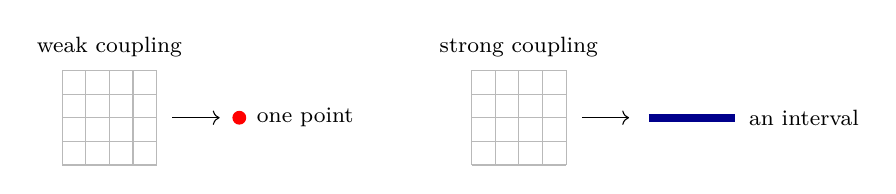
\begin{tikzpicture}
  \node at (0.6,1.5){\footnotesize weak coupling};
  \draw[step=0.3,gray!55] (0,0) grid (1.2,1.2);
  \draw[->](1.4,0.6)--(2.0,0.6);
  \fill[red](2.25,0.6)circle(2.5pt); \node[right] at(2.35,0.6){\footnotesize one point};
  \begin{scope}[shift={(5.2,0)}]
    \node at (0.6,1.5){\footnotesize strong coupling};
    \draw[step=0.3,gray!55] (0,0) grid (1.2,1.2);
    \draw[->](1.4,0.6)--(2.0,0.6);
    \draw[blue!55!black,line width=3pt](2.25,0.6)--(3.35,0.6); \node[right] at(3.4,0.6){\footnotesize an interval};
  \end{scope}
\end{tikzpicture}}

\item \textbf{Exchangeability / mixture readout.}\footnote{Lean: the imprecise
de Finetti mixing-family in
\lpath{Mettapedia/Logic/DeFinettiProjectiveCredalBridge.lean}; see
Appendix~\ref{app:formal}, item~\ref{item:exch}.} An order-free stream has a
canonical mixture forecast, but the raw all-questions law depends on the
compatibility boundary of Section~\ref{sec:exch}. \emph{Trap:} demanding every
mixture component be degenerate, which wrongly rejects legitimate
``unsure-of-the-bias'' families.

\knobpic{%
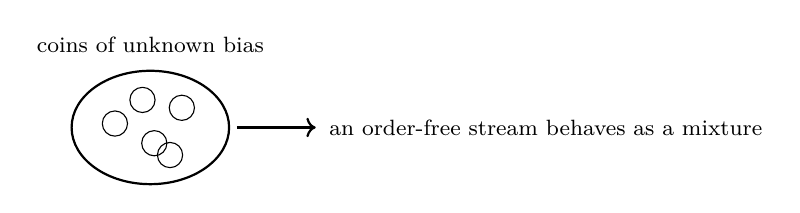
\begin{tikzpicture}
  \draw[thick] (0,0) ellipse (1.0 and 0.72);
  \foreach \x/\y in {-0.45/0.05, 0.05/-0.2, 0.4/0.25, -0.1/0.35, 0.25/-0.35}{\draw (\x,\y) circle (0.16);}
  \node at (0,1.05){\footnotesize coins of unknown bias};
  \draw[->,thick](1.1,0)--(2.1,0);
  \node[right] at (2.15,0){\footnotesize an order-free stream behaves as a mixture};
\end{tikzpicture}}

\item \textbf{Rule-level confidence transport (revision).}\footnote{Lean:
\lid{transportedConfidenceRevision} and \lid{plnConfidenceRevision} in
\lpath{Mettapedia/Logic/PLNConfidenceWeightRevision.lean}.} Combining two
independent bodies of evidence is ``add the counts, then re-read,'' not ``average
the confidences.'' $(4,2)\oplus(3,1)=(7,3)$ gives $\STV{0.7}{0.909}$ --- higher
than either source ($\STV{0.667}{0.857}$ and $\STV{0.75}{0.800}$). \emph{Trap:}
averaging displayed confidences, which absurdly \emph{lowers} confidence after
seeing \emph{more} evidence.

\knobpic{%
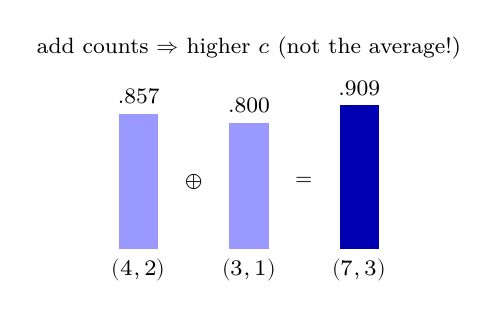
\begin{tikzpicture}
  \fill[blue!40](0,0) rectangle (0.5,1.71); \node[below] at(0.25,0){\footnotesize $(4,2)$};\node[above] at(0.25,1.71){\footnotesize .857};
  \node at (0.95,0.85){\footnotesize $\oplus$};
  \fill[blue!40](1.4,0) rectangle (1.9,1.6); \node[below] at(1.65,0){\footnotesize $(3,1)$};\node[above] at(1.65,1.6){\footnotesize .800};
  \node at (2.35,0.85){\footnotesize $=$};
  \fill[blue!70!black](2.8,0) rectangle (3.3,1.82); \node[below] at(3.05,0){\footnotesize $(7,3)$};\node[above] at(3.05,1.82){\footnotesize .909};
  \node[align=center] at (1.65,2.55){\footnotesize add counts $\Rightarrow$ higher $c$ (not the average!)};
\end{tikzpicture}}

\item \textbf{Provenance / route.}\footnote{Lean:
\lid{route\_kappa\_changes\_confidence\_not\_strength} in
\lpath{Mettapedia/Logic/PLNConfidenceDoFCanary.lean}.} Same counts, different route, route-specific
confidence. From $(3,0)$: strength $1.0$ on every route, but confidence $0.75$ on
a direct route ($\kappa=1$) versus $0.273$ on a pathway-mediated route
($\kappa=8$). \emph{Trap:} merging routes before applying route-specific
$\kappa$, destroying both the audit trail and the discount.

\knobpic{%
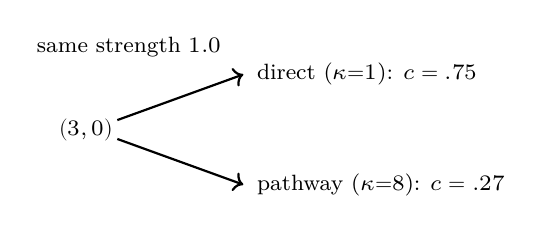
\begin{tikzpicture}
  \node (s) at (0,0){\footnotesize $(3,0)$};
  \draw[->,thick](0.4,0.12)--(2.0,0.7); \node[right] at(2.05,0.7){\footnotesize direct ($\kappa{=}1$): $c=.75$};
  \draw[->,thick](0.4,-0.12)--(2.0,-0.7); \node[right] at(2.05,-0.7){\footnotesize pathway ($\kappa{=}8$): $c=.27$};
  \node at (0.55,1.05){\footnotesize same strength $1.0$};
\end{tikzpicture}}

\item \textbf{Extra structure beyond $\STV{s}{c}$.}\footnote{Lean:
\lid{phase\_not\_visible\_to\_standard\_pln\_view} in
\lpath{Mettapedia/Logic/PLNAmplitudePhase.lean}.} Some beliefs carry more than
strength and confidence --- a ``phase'' or dependence witness --- and two beliefs
with identical $\STV{s}{c}$ can differ once a composition rule that \emph{sees}
the extra coordinate is in play. \emph{Trap:} both carrying phase needlessly in a
plain classifier, \emph{and} assuming $\STV{s}{c}$ is complete when
interference-like composition matters.
\knobpic{%
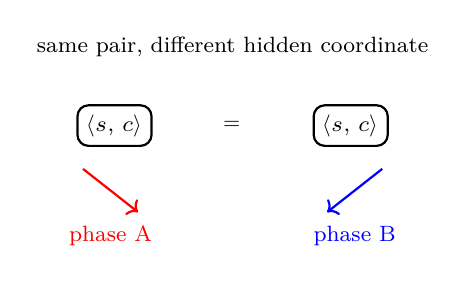
\begin{tikzpicture}
  \node[draw,rounded corners,thick] (a) at (0,0){\footnotesize $\STV{s}{c}$};
  \node[draw,rounded corners,thick] (b) at (3,0){\footnotesize $\STV{s}{c}$};
  \node at (1.5,0.0){\footnotesize $=$};
  \draw[->,red,thick](-0.4,-0.55)--(0.3,-1.1); \node[red,below] at(-0.05,-1.15){\footnotesize phase A};
  \draw[->,blue,thick](3.4,-0.55)--(2.7,-1.1); \node[blue,below] at(3.05,-1.15){\footnotesize phase B};
  \node at (1.5,1.0){\footnotesize same pair, different hidden coordinate};
\end{tikzpicture}}

\end{enumerate}

The thread through all nineteen: a degree of freedom is a place where a
\emph{convention} masquerades as a \emph{fact}. Naming them is what lets you
choose deliberately --- and lets two honest modellers reconcile beliefs that
print the same two numbers.

\section{Conclusion}\label{sec:conclusion}

PLN's truth value is two numbers standing in for a whole set of admissible
probabilities. Strength is the centre of the set on the question you ask;
confidence falls with the set's width. The two numbers tell the whole story
exactly when the set pins your question to a point, and report a genuine interval
otherwise --- one fork, recurring from a single coin up to infinite interacting
systems. Freedom hides in three places: the width you chose (visible), the
world's single hidden pick (invisible, and rightly so), and the structure's own
non-uniqueness in the infinite limit (visible, as real width). And nineteen
everyday modelling choices live in the gap between ``the two numbers'' and ``the
set behind them.'' Every claim here has a machine-checked counterpart
(Appendix~\ref{app:formal}) and a runnable demonstration
(Appendix~\ref{app:run}).

\section{Related work}\label{sec:related}

\paragraph{Imprecise probability.} The credal-set / lower-prevision picture ---
a belief as a \emph{set} of distributions, summarized by lower and upper
expectations --- is Walley's~\cite{walley91}. Our ``spread,'' ``pinned versus
range,'' and the read-off of strength and confidence are the PLN-facing form of
his coherent lower previsions and their envelopes.

\paragraph{Exchangeability.} de Finetti's theorem~\cite{definetti37} is the
classical bridge: an exchangeable (order-free) infinite sequence is a mixture of
i.i.d.\ trials. Section~\ref{sec:exch} is the imprecise version --- a \emph{set}
of such mixtures, with the compatibility boundary that decides when finite
forecasts extend to one whole-process law.

\paragraph{Infinite systems.} The Dobrushin--Lanford--Ruelle
framework~\cite{dobrushin68,lanford-ruelle69} characterizes infinite Gibbs
measures by their finite-volume conditionals; Dobrushin's uniqueness condition is
the ``weak coupling, one answer'' result of Section~\ref{sec:weak}, and
phase-transition non-uniqueness is the ``strong coupling, an interval'' result of
Section~\ref{sec:strong}. Markov logic networks~\cite{richardson-domingos06,
singla-domingos05} are the logic-facing instance: weighted clauses specifying a
distribution over possible worlds.

\paragraph{Sibling papers.} This note is a companion to \xiPLN\ and the PLN
Review (\lpath{papers/xiPLN.tex}, \lpath{papers/pln-review.tex}), which treat the
evidence algebra and PLN's inference rules; the WM-PLN book~\cite{wmpln-book}
contains the informal predecessor of the degrees-of-freedom discussion this paper
makes precise.

\appendix

\section{Run it yourself}\label{app:run}

Every number in the body is reproduced by a small runnable companion pack at
\lpath{papers/pln-confidence-examples/}. It runs on two independent MeTTa engines
(CeTTa in its HE mode, and PeTTa), so the arithmetic is not taking any one
implementation's word for it.

\begin{verbatim}
cd papers/pln-confidence-examples
sh run_all.sh        # build CeTTa, run every dofNN, then PeTTa
\end{verbatim}

The pack has one small example per degree of freedom (\lpath{metta/dof01..18}),
each a self-contained file ending in queries whose printed outputs are the
claims; a one-line-per-knob index (\lpath{README.md}); and the expected numbers
for a human spot-check. The honest contract is stated there and bears repeating:
\textbf{the Lean theorems of Appendix~\ref{app:formal} are the correctness
oracle; the \texttt{.metta} runs are intuition and reproducibility, never proof.}
Matching output is an illustration check, not a verification.

A few entries (the infinite-boundary ones --- exchangeable streams, weak/strong
coupling, completion extreme points, hidden phase) have no finite executable that
could settle the claim; for those the pack ships the closest finite ``shadow''
(e.g.\ the Laplace forecast of Section~\ref{sec:exch}) and points at the theorem
that carries the real content. The index marks each row as \emph{runnable},
\emph{structural} (a finite shadow), or \emph{theorem-only}, so nothing
infinite masquerades as something you can compute.

\section{Formal companion: the statements, de-jargoned}\label{app:formal}

The body avoided machinery on purpose. Here are the load-bearing statements, each
as: the plain-English claim the body relied on, the machine-checked Lean name,
and one line on what it forces. All are verified in the Mettapedia Lean library;
the public entry point bundling them is
\lid{confidenceCharacterizationEndpointProfile}, and the names below are live
declarations in that development. The core objects: a \emph{gamble} is a
real-valued function on the outcome space (a random variable / payoff); a
\emph{precise prevision} is an expectation operator $E[\cdot]$ on gambles; a
\emph{credal set} (our ``spread'') is a set of these; the \emph{lower} and
\emph{upper envelopes} are the pointwise $\inf$ and $\sup$ of $E[X]$ over the set
--- the endpoints $L$ and $U$. The listings are lightly ASCII-formatted
(\code{Omega} for $\Omega$, \code{->} for $\to$, and \code{forall}/\code{exists}/%
\code{in}/\code{and}/\code{not} for the binders and connectives). The source
files are \lpath{Mettapedia/ProbabilityTheory/ImpreciseProbability/ProjectiveCredal.lean}
(the credal stack), \lpath{Mettapedia/Logic/DeFinettiProjectiveCredalBridge.lean},
\lpath{Mettapedia/Logic/MarkovLogicInfiniteCredalBridge.lean}, and
\lpath{Mettapedia/Logic/MarkovLogicInfiniteSymmetricGridExample.lean}.

\begin{enumerate}
\item \textbf{The read-off.} Strength is the midpoint and confidence a decreasing
function $g$ of the width of $[L,U]$. The midpoint and $g$ are interface
choices; none of the results below depends on them. \emph{Forces:} the meaning of
$\STV{s}{c}$ as centre-and-width of an envelope interval.
\begin{lstlisting}
abbrev CredalPrevisionSet (Omega : Type*) := Set (PrecisePrevision Omega)

def lowerEnvelope (C : CredalPrevisionSet Omega) (X : Gamble Omega) : Real :=
  sInf ((fun P : PrecisePrevision Omega => P X) '' C)
def upperEnvelope (C : CredalPrevisionSet Omega) (X : Gamble Omega) : Real :=
  sSup ((fun P : PrecisePrevision Omega => P X) '' C)
\end{lstlisting}

\item\label{item:dich} \textbf{The pinned/range dichotomy (the spine).} If every
admissible prevision assigns $X$ the same value the envelopes coincide; if two
disagree the envelope strictly opens; and the two cases are mutually exclusive.
\emph{Forces:} Section~\ref{sec:fork} --- pinned and range are the only cases and
cannot coexist.
\begin{lstlisting}
def credalSetDetermines (C : CredalPrevisionSet Omega) (X : Gamble Omega) : Prop :=
  forall P : PrecisePrevision Omega, P in C ->
    forall Q : PrecisePrevision Omega, Q in C -> P X = Q X
def credalSetHasStrictWidth (C : CredalPrevisionSet Omega) (X : Gamble Omega) : Prop :=
  exists P : PrecisePrevision Omega, P in C and
    exists Q : PrecisePrevision Omega, Q in C and P X < Q X

theorem not_credalSetDetermines_of_strictWidth
    (hWidth : credalSetHasStrictWidth C X) : not (credalSetDetermines C X)

theorem lower_eq_upperEnvelope_of_credalSetDetermines
    (C : CredalPrevisionSet Omega) (X : Gamble Omega) (hC : C.Nonempty)
    (hBddBelow : BddBelow ((fun P => P X) '' C))
    (hBddAbove : BddAbove ((fun P => P X) '' C))
    (hP : P in C) (hDet : credalSetDetermines C X) :
    lowerEnvelope C X = upperEnvelope C X

theorem lower_upperEnvelope_nontrivial_of_strictWidth
    (C : CredalPrevisionSet Omega) (X : Gamble Omega)
    (hBddBelow : BddBelow ((fun P => P X) '' C))
    (hBddAbove : BddAbove ((fun P => P X) '' C))
    (hWidth : credalSetHasStrictWidth C X) :
    lowerEnvelope C X < upperEnvelope C X
\end{lstlisting}

\item \textbf{Finite totality.} On a finite outcome space the construction never
misbehaves --- the spread avoids sure loss and is coherent --- and a one-element
spread pins every question. \emph{Forces:} the map from a specification to
$\STV{s}{c}$ is well defined.
\begin{lstlisting}
theorem lowerEnvelopePrevision_avoidsSureLoss_of_finite
    [Fintype Omega] [Nonempty Omega]
    (C : CredalPrevisionSet Omega) (hC : C.Nonempty)
    (hBdd : forall X, BddBelow ((fun P => P X) '' C)) :
    (lowerEnvelopePrevision C hC hBdd).avoidsSureLoss

theorem lowerEnvelope_singleton (P : PrecisePrevision Omega) (X : Gamble Omega) :
    lowerEnvelope ({P} : CredalPrevisionSet Omega) X = P X
\end{lstlisting}

\item\label{item:global} \textbf{The dichotomy lifts to built-up specs.} For
beliefs glued from local windows, the same fork holds globally. \emph{Forces:}
Section~\ref{sec:build}.
\begin{lstlisting}
def determinesGlobalGamble
    (S : ProjectiveLocalCredalSpec Window Global) (X : Gamble Global) : Prop :=
  credalSetDetermines S.projectiveLimitCredalSet X
def hasStrictGlobalWidth
    (S : ProjectiveLocalCredalSpec Window Global) (X : Gamble Global) : Prop :=
  credalSetHasStrictWidth S.projectiveLimitCredalSet X

theorem not_determinesGlobalGamble_of_strictWidth
    (S : ProjectiveLocalCredalSpec Window Global)
    (hWidth : S.hasStrictGlobalWidth X) : not (S.determinesGlobalGamble X)
\end{lstlisting}

\item\label{item:exch} \textbf{Order-free streams.} The canonical mixture
forecast always exists; the stronger ``one consistent law for every question''
holds \emph{exactly} when a respecting lower prevision exists. It may \emph{not}
be tightened to ``every mixture component degenerate'' --- that strengthening is
refuted. \emph{Forces:} the takeaway and caution of Section~\ref{sec:exch}.
\begin{lstlisting}
theorem impreciseDeFinetti_analyticMixingFamily_
    sharpCompatibilityCrown
    (C : Set BernoulliMixture) (hC : C.Nonempty) :
    ImpreciseDeFinettiCanonicalExternalMixingFamily C hC and
      (ImpreciseDeFinettiAnalyticMixingFamilyProcessLawCrown C hC <->
        exists L : LowerPrevision (Nat -> Bool),
          (bernoulliMixturePrefixProcessLowerSpec C
            (fun M _ n => bernoulliMixturePrefixLaw_analytic M n) hC).respectsLocalLower L)

theorem not_forall_impreciseDeFinetti_
    analyticMixingFamilyProcessLawCrown_imp_
    pointwiseZeroInterior_closed :
    not (forall (C : Set BernoulliMixture) (hC : C.Nonempty),
        ImpreciseDeFinettiAnalyticMixingFamilyProcessLawCrown C hC ->
          AnalyticMixingFamilyPointwiseZeroInterior C)
\end{lstlisting}

\item\label{item:weak} \textbf{Weak coupling collapses.} Under a uniform
small-influence budget every finite query is pinned, and the global model is
unique. We prove only this direction; the converse (budget failure forcing
width) is not claimed. \emph{Forces:} Section~\ref{sec:weak}, top of the fork.
\begin{lstlisting}
theorem dlrQueryDetermined_of_uniform
    (M : ClassicalInfiniteGroundMLNSpec Atom ClauseId)
    (hM : M.PaperUniformSmallTotalInfluence) (q : ConstraintQuery Atom) :
    dlrQueryDetermined M q

theorem infiniteMLN_queryEnvelope_precise_of_uniform
    (M : ClassicalInfiniteGroundMLNSpec Atom ClauseId)
    [Nonempty (DLRCompletion M)]
    (hM : M.PaperUniformSmallTotalInfluence) (q : ConstraintQuery Atom) :
    infiniteMLNLowerQueryEnvelope M q = infiniteMLNUpperQueryEnvelope M q
\end{lstlisting}

\item\label{item:strong} \textbf{Strong coupling keeps an interval.} A
low-temperature two-dimensional symmetric grid has an origin query with genuinely
positive envelope width (so confidence is strictly below its ceiling), a range
the distant boundary controls --- and this is proved with \emph{no} hypotheses.
The two stuck magnets are the finite witness used in the body. \emph{Forces:}
Section~\ref{sec:strong}, bottom of the fork.
\begin{lstlisting}
-- the crown asserts, for the zero-field grid at coupling w:
structure SymmetricGridZeroFieldOriginPLNStrictIntervalCrown
    (w : Real) : Prop where
  queryEnvelopeWidth_pos :
    0 < infiniteMLNQueryEnvelopeWidth
          (symmetricGridZeroFieldClassicalSpec w) gridOriginSpinUpQuery
  queryEnvelopeWidthComplement_lt_one :
    infiniteMLNQueryEnvelopeWidthComplement
          (symmetricGridZeroFieldClassicalSpec w) gridOriginSpinUpQuery < 1
  queryOutcomeCredalSet_width_pos : ...   -- the binary outcome has positive width

-- proved with no hypotheses at coupling w = 24:
theorem symmetricGridZeroField_originPLNStrictIntervalCrown_of_
    axisAnchoredContourCode_twentyFour :
    SymmetricGridZeroFieldOriginPLNStrictIntervalCrown (24 : Real)

-- the finite witness used in the body (two stuck magnets):
theorem twoSpinMagnetEnvelope_nontrivial :
    lowerEnvelope twoSpinMagnetCredalSet twoSpinFirstUpGamble <
      upperEnvelope twoSpinMagnetCredalSet twoSpinFirstUpGamble
\end{lstlisting}

\item \textbf{Three freedoms, formally.} The sharpest negative claim of the
paper: $\STV{s}{c}$ is a property of the credal \emph{set}, so the world's single
choice of member (source (B)) cannot change it, while the spec width (A) and
structural non-uniqueness (C) can. This is the content of items
\ref{item:dich}--\ref{item:strong} read together, and is why source (B) is
invisible in Figure~\ref{fig:three}.
\end{enumerate}

The full type definitions and proof scripts (the credal stack, the projective
construction, the DLR specialization, and the contour argument behind
item~\ref{item:strong}) live in the Lean sources under
\lpath{lean/mettapedia/Mettapedia/}; this appendix states what they establish,
not how. The companion package's \lpath{lean/DOF-LEAN-MAP.md} maps each
degree of freedom in Section~\ref{sec:zoo} to its specific theorem.

\begin{thebibliography}{10}

\bibitem{walley91}
Peter Walley.
\newblock \emph{Statistical Reasoning with Imprecise Probabilities}.
\newblock Chapman \& Hall, 1991.

\bibitem{definetti37}
Bruno de Finetti.
\newblock La pr\'evision: ses lois logiques, ses sources subjectives.
\newblock \emph{Annales de l'Institut Henri Poincar\'e}, 7:1--68, 1937.

\bibitem{dobrushin68}
R.\ L.\ Dobrushin.
\newblock Description of a random field by means of conditional
        probabilities and conditions of its regularity.
\newblock \emph{Theory of Probability and its Applications},
        13(2):197--224, 1968.

\bibitem{lanford-ruelle69}
O.\ Lanford and D.\ Ruelle.
\newblock Observables at infinity and states with short-range correlations
        in statistical mechanics.
\newblock \emph{Communications in Mathematical Physics}, 13:194--215, 1969.

\bibitem{richardson-domingos06}
Matthew Richardson and Pedro Domingos.
\newblock Markov logic networks.
\newblock \emph{Machine Learning}, 62:107--136, 2006.

\bibitem{singla-domingos05}
Parag Singla and Pedro Domingos.
\newblock Discriminative training of Markov logic networks.
\newblock In \emph{AAAI 2005}.

\bibitem{goertzel-pln}
Ben Goertzel, Matthew Ikl\'e, Izabela Goertzel, and Ari Heljakka.
\newblock \emph{Probabilistic Logic Networks: A Comprehensive Framework
        for Uncertain Inference}.
\newblock Springer, 2008.

\bibitem{xipln}
Mettapedia Working Notes.
\newblock $\xi$PLN: a correct and complete foundation for probabilistic
        logic networks.
\newblock In the Mettapedia corpus: \lpath{papers/xiPLN.tex}.

\bibitem{wmpln-book}
Mettapedia Working Notes.
\newblock The WM-PLN book.
\newblock In the Mettapedia corpus: \lpath{papers/wm-pln-book.tex}.

\bibitem{pln-review}
Mettapedia Working Notes.
\newblock PLN review and corrections.
\newblock In the Mettapedia corpus: \lpath{papers/pln-review.tex}.

\end{thebibliography}

\end{document}
